
\subsection{tempOnDay()}
The first of the proposed graphs was a histogram that will show all the temperatures recorded over the years for a single day. The member function of tempTrender that deoes this was called "tempOnDay()".\par
There are two variants proposed for the tempOnDay member function in the instructions file: one that takes two int values as input (month and day) and one that takes a number between 0 and 365, corresponding to a specific day of the year. We implemented both.\par

\begin{figure}[h]
\centering
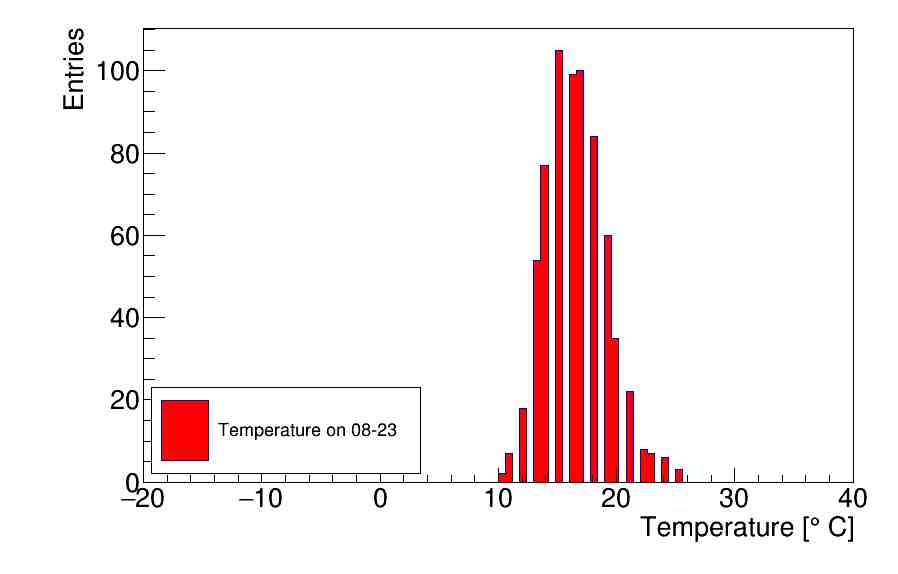
\includegraphics[scale=0.3]{graph1.png}
\caption{Temperature for a specific day. Histogram produce by tempOnDay(month, day) }
\end{figure}